\documentclass[12pt, a4paper]{article}

\usepackage[utf8]{inputenc}
\usepackage[T1]{fontenc}
\usepackage[brazilian]{babel}
\usepackage{mathptmx}
\usepackage{amsmath, amssymb}
\usepackage{graphicx}
\usepackage{booktabs}
\usepackage{geometry}
\usepackage{float}
\usepackage{setspace}
\usepackage{caption}

\geometry{top=3cm, bottom=2cm, left=3cm, right=2cm}
\setstretch{1.5}
\captionsetup{font=small, labelfont=bf, labelsep=endash}

\begin{document}

\begin{center}
    \Large\textbf{Resultados e Discussão: A Arquitetura DataOps sob Estresse} \\[0.5cm]
    \normalsize\textbf{Projeto DataOps / UNIFEI} \\
    \small{\today}
\end{center}

\vspace{0.5cm}
\noindent\rule{\textwidth}{1pt}

\section{O Desafio Físico e a Metodologia de Estresse}
A consolidação de um ecossistema analítico orientado a eventos (\textit{Event-Driven}) para o monitoramento geoespacial demanda uma validação rigorosa de sua capacidade de resposta sob estresse. A base de dados transacional coligida durante as simulações consolidou um montante de $\sim$3,1 milhões de registros de focos de calor espaciais. 

Contudo, a natureza intrínseca da ingestão contínua assíncrona (\textit{Streaming}) via Apache Kafka originou uma patologia de armazenamento conhecida como \textit{Tiny Segments} (Segmentos Minúsculos). Os dados assentaram-se no \textit{Deep Storage} fragmentados em exatos 6.518 arquivos distintos, totalizando cerca de 211 MB. Esta fragmentação extrema formou a linha de base empírica para testar a escalabilidade do motor Apache Druid.

\section{A Ilusão da Escalabilidade Vertical}
A primeira fase da experimentação visou responder à seguinte premissa: \textit{"A injeção de força computacional bruta (Hardware Tuning) é capaz de mitigar a fragmentação de disco?"}. Para tal, orquestraram-se três cenários progressivos utilizando \textit{Cgroups} do Docker, alocando-se 2, 4 e 6 núcleos lógicos do processador.

Os resultados evidenciaram uma curva clássica de rendimentos decrescentes (Lei de Amdahl). Conforme ilustrado na Figura 1, saltar de 2 para 4 núcleos reduziu a latência média de leitura bruta (\textit{Cold Start}) quase pela metade (de $\sim$4.091 ms para $\sim$2.319 ms). Contudo, a alocação máxima de 6 núcleos esbarrou em um teto sistêmico, travando o ecossistema na faixa dos $\sim$1.624 ms. A escalabilidade da CPU tornou-se inócua perante o insuperável gargalo de Entrada/Saída (\textit{I/O Overhead}) gerado pela abertura e fechamento de 6.518 arquivos sequenciais.

\begin{figure}[H]
\centering
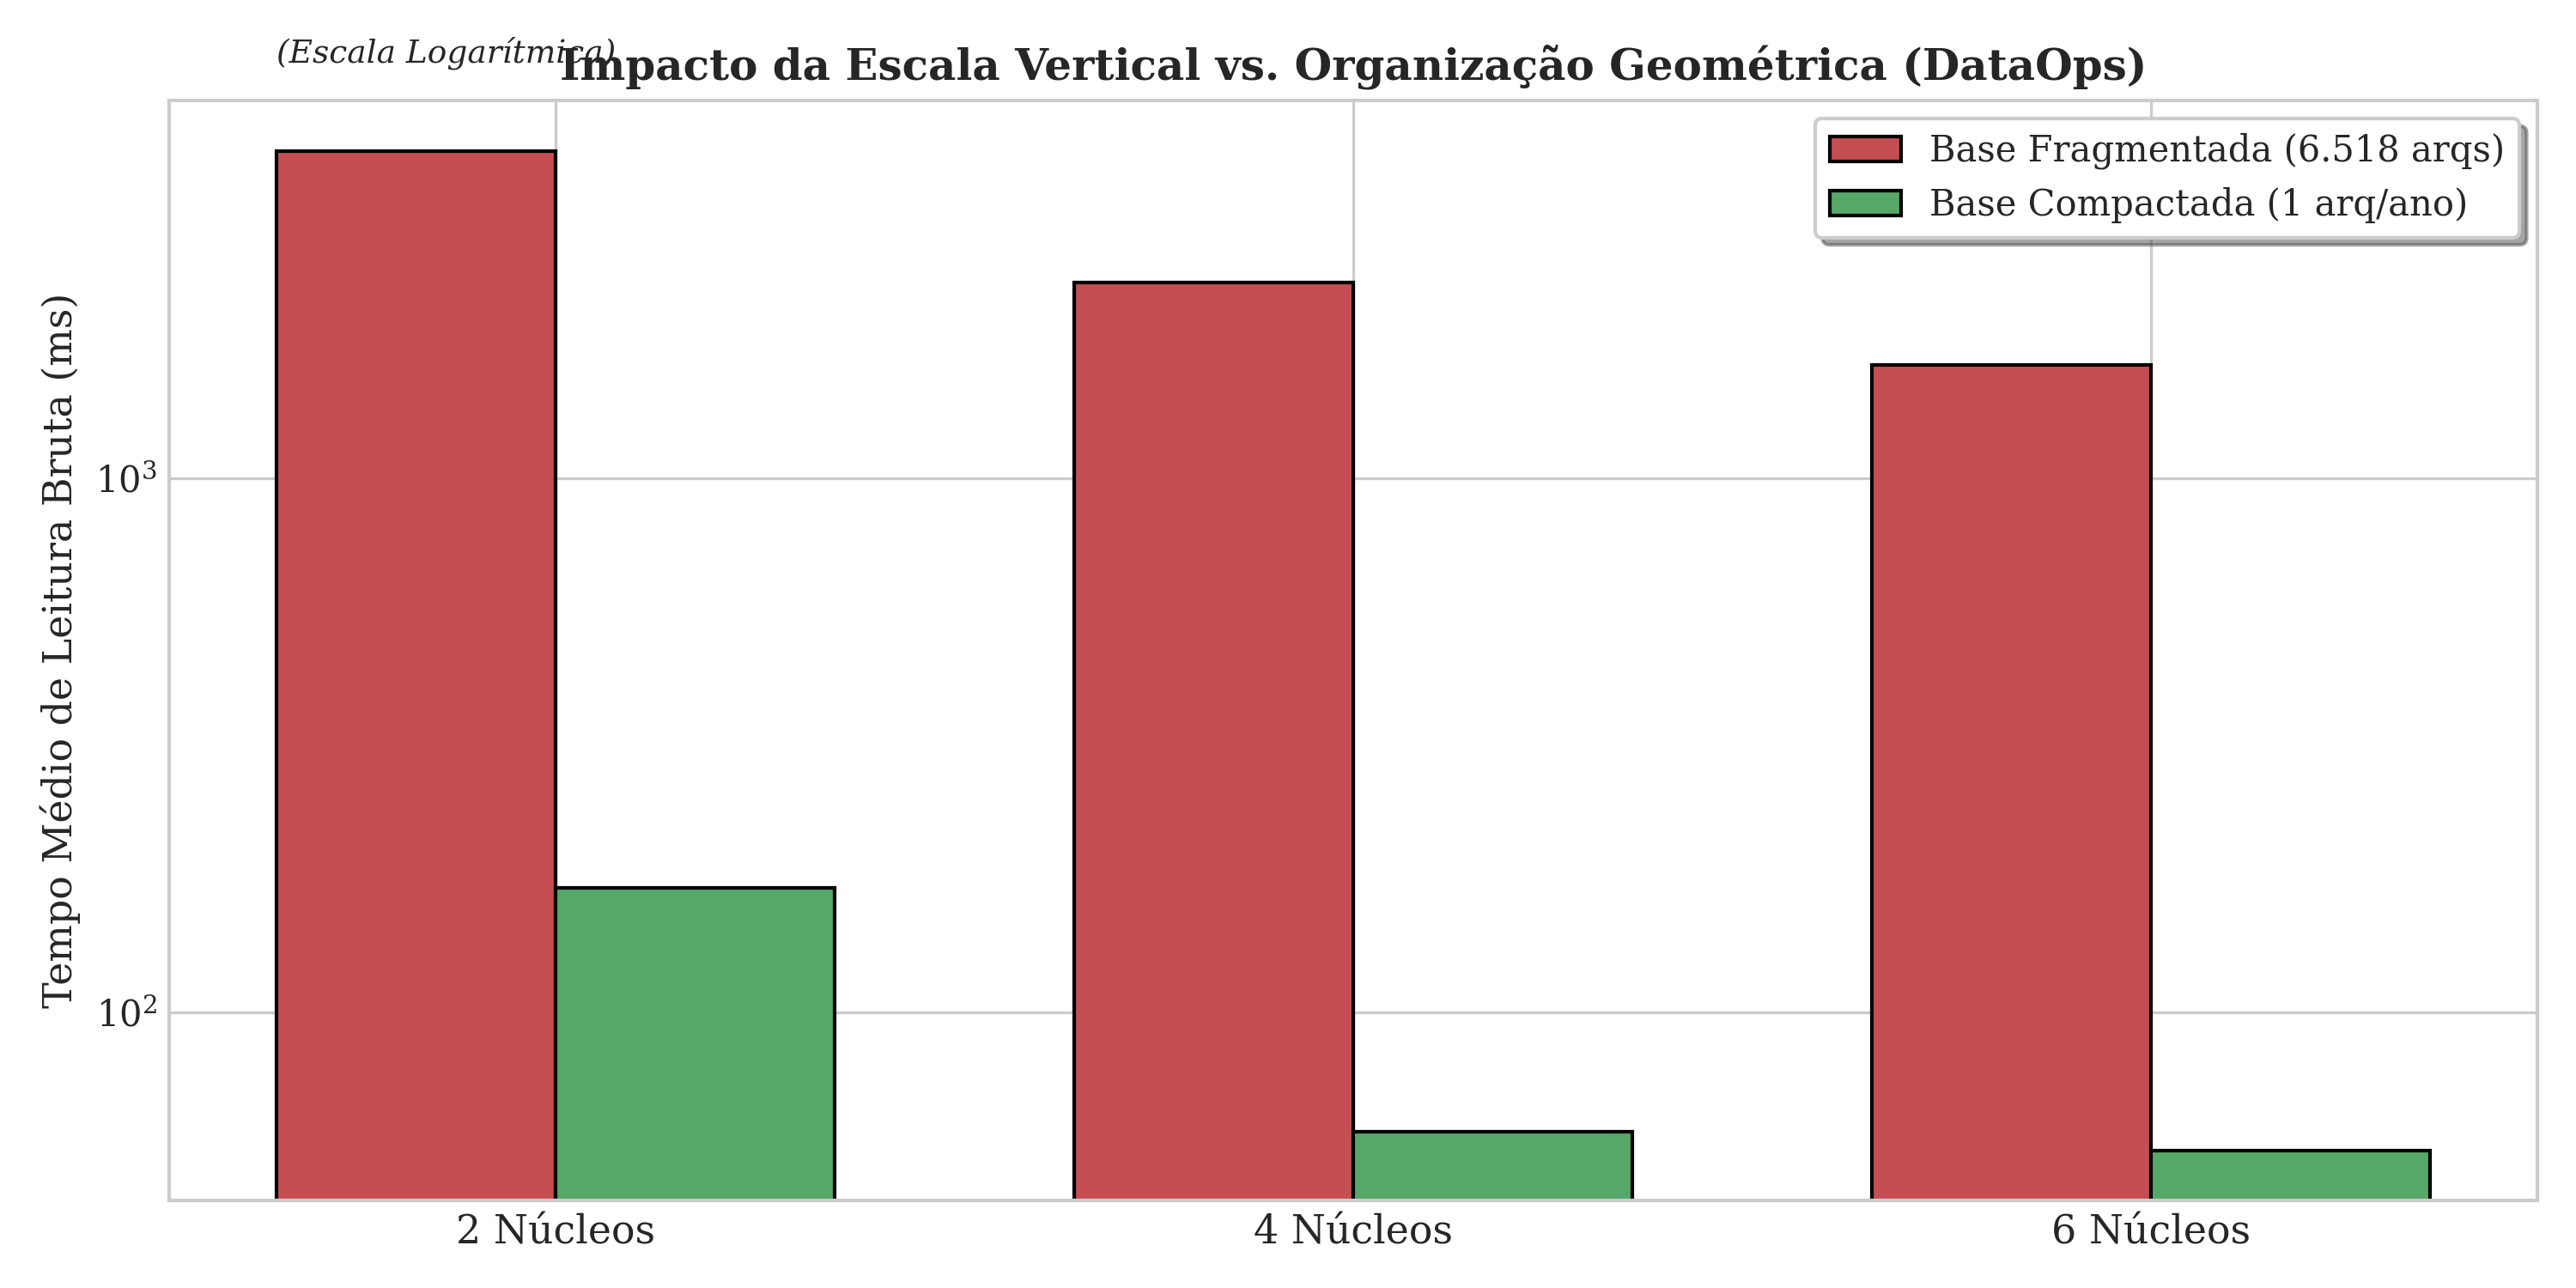
\includegraphics[width=0.9\textwidth]{tcc_fig1_evolucao_cold.png}
\caption{Comparativo Logarítmico: A estagnação da CPU perante a fragmentação versus a eficiência imediata da base compactada.}
\end{figure}

\section{Autópsia do ``Paradoxo do Cache''}
A descoberta mais contundente da fase de estrangulamento ocorreu na camada de Memória RAM Volátil. Teoricamente, o mecanismo de \textit{Cache} de um motor OLAP deve fornecer respostas instantâneas ao interceptar requisições mapeadas. Todavia, registrou-se o fenômeno aqui cunhado como \textbf{Paradoxo do Cache}.

Em leituras de alta restrição territorial (Filtros Complexos da FUNAI), a memória apresentou \textbf{latência negativa extrema}. Com 6 núcleos ativos, a leitura do cache atrasou a resposta em -12,47\% quando comparada à varredura direta do disco.

\begin{figure}[H]
\centering
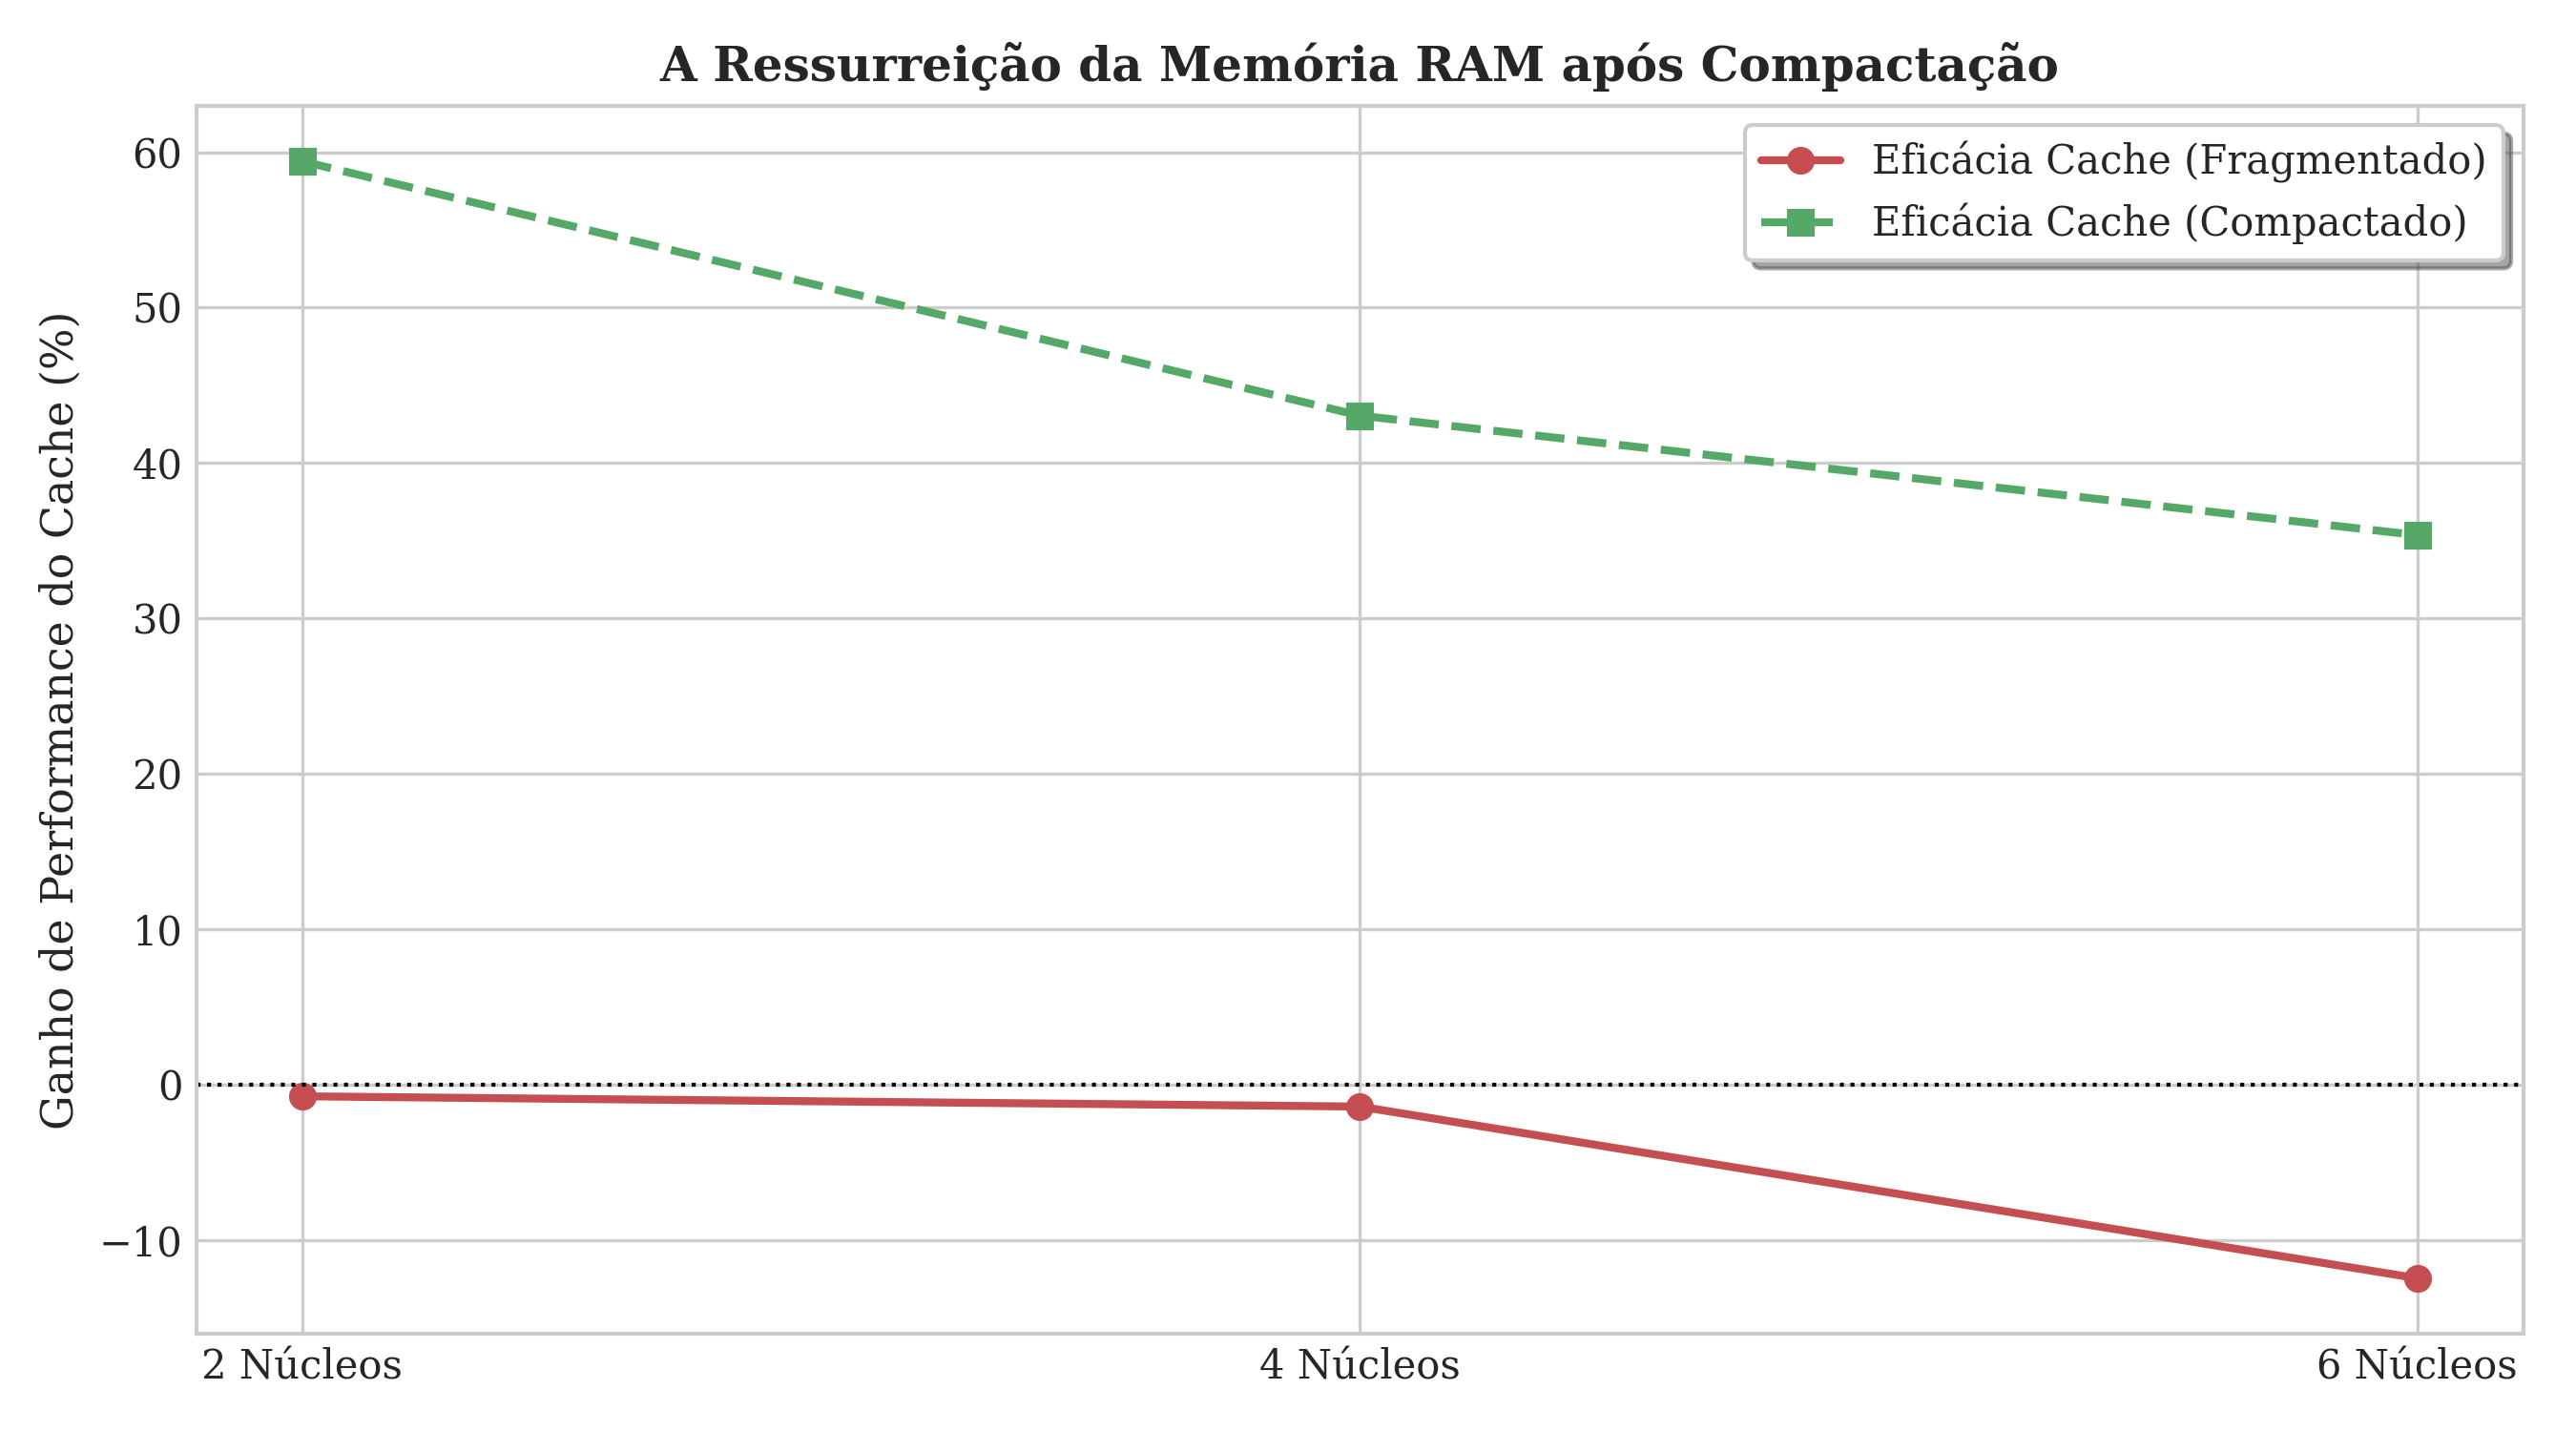
\includegraphics[width=0.9\textwidth]{tcc_fig2_paradoxo_cache.png}
\caption{Eficácia da Memória RAM: O colapso na base fragmentada e a ressurreição após compactação geométrica.}
\end{figure}

Isto comprova matematicamente que a Unidade Lógica e Aritmética (ULA) colapsa não por falta de poder de cálculo temporal, mas pela exaustão logística de instanciar, indexar e fundir (\textit{merge}) os metadados de 6.518 estilhaços na memória em frações de milissegundo. O processador "engasga" na tentativa de montar o quebra-cabeça do cache.

\vspace{1cm}
\begin{center}
\textit{--- Fim da Parte 1 ---} \\
\textit{(Na próxima seção detalharemos a vitória da Compactação!)}
\end{center}

\end{document}
